\section{Środowisko testowe}
\label{sec:testing}
    Podczas budowy dowolnego systemu, niezwykle ważne jest testowanie elementów składowych.
    Połączone moduły również wymagają sprawdzenia ich współpracy.
    W informatyce kontrolę oprogramowania zapewniają testy jednostkowe, które weryfikują działanie poszczególnych algorytmów i programów.
    Natomiast w przypadku prac nad sprzętem niezbędne jest zbudowanie odpowiedniego środowiska, pozwalającego na testowanie każdego elementu osobno oraz łącznie poszczególnych podzespołów w bloki funkcjonalne.
    Dlatego wykonanie fizyczne należy podzielić na kilka etapów, opisanych poniżej:
    \begin{enumerate}
        \item Budowa prototypu na płytce stykowej.
        \item Złożenie ramy pojazdu z elektroniką umieszczoną na płytce stykowej wraz z doprowadzonym zewnętrznym zasilaniem.
        \item Sprawdzenie działania pojazdu z płytką stykową zasilaną bateryjnie.
        \item Wykonanie płytki prototypowej z połączeniami wszystkich elementów na stałe ponownie z zewnętrznym zasilaniem.
        \item Sprawdzenie działania prototypu pojazdu z zasilaniem akumulatorowym.
    \end{enumerate}
    Każdy z wymienionych kroków charakteryzował się innym rodzajem testów oraz własnymi problemami.
    Zakończenie jednej fazy i przejście do następnej było możliwe dopiero po uznaniu przez autora, że układ pracuje poprawnie.

    \subsection{Modele prototypowe}
        Pierwszym etapem było zbudowanie na podstawie schematu z rysunku \ref{schema:block} modelu elektronicznego na płytce stykowej.
        Poniżej przedstawiono zdjęcie układu złożonego w ten sposób.
        Obwód ten pozwalał na bezpieczne testowanie nowych funkcji, bez ryzyka uszkodzenia elementów.
        Dodatkowymi zaletami takiego połączenia są: możliwość bezpośredniego debugowania kodu oraz szybka wymiana modułów w przypadku konfliktów między poszczególnymi blokami.
        \begin{figure}[!ht]
            \centering
            \includegraphics[width = 0.7\textwidth, trim = {500px, 500px, 350px, 350px}, clip]{Breadboard.jpg}
            \caption{Model prototypowy na płytce stykowej}
            \label{fig:breadboard}
        \end{figure}

        Tak zbudowany obwód działał bez zarzutu, dzięki czemu możliwe było przejście do następnej fazy pracy.

        W tym celu system z rysunku \ref{fig:breadboard} został skompresowany, aby zmieścił się na pojedynczej mniejszej płytce.
        Następnie układ zamocowano na samochodzie.
        Do tego celu zaprojektowano obudowę, którą przykręcono do całości, po czym umieszczono w niej zminiaturyzowany system.
        Na zdjęciu poniżej (rys. \ref{fig:breadboard_car}) przedstawiono opisaną sytuację.

        Pojazd wyposażono w dwa pojedyncze koszyki na akumulatory oraz moduł BMS (Battery Management System).
        Dzięki temu całość mogła pracować na zasilaniu bateryjnym bez obawy o uszkodzenia.

        \begin{figure}[!ht]
            \centering
            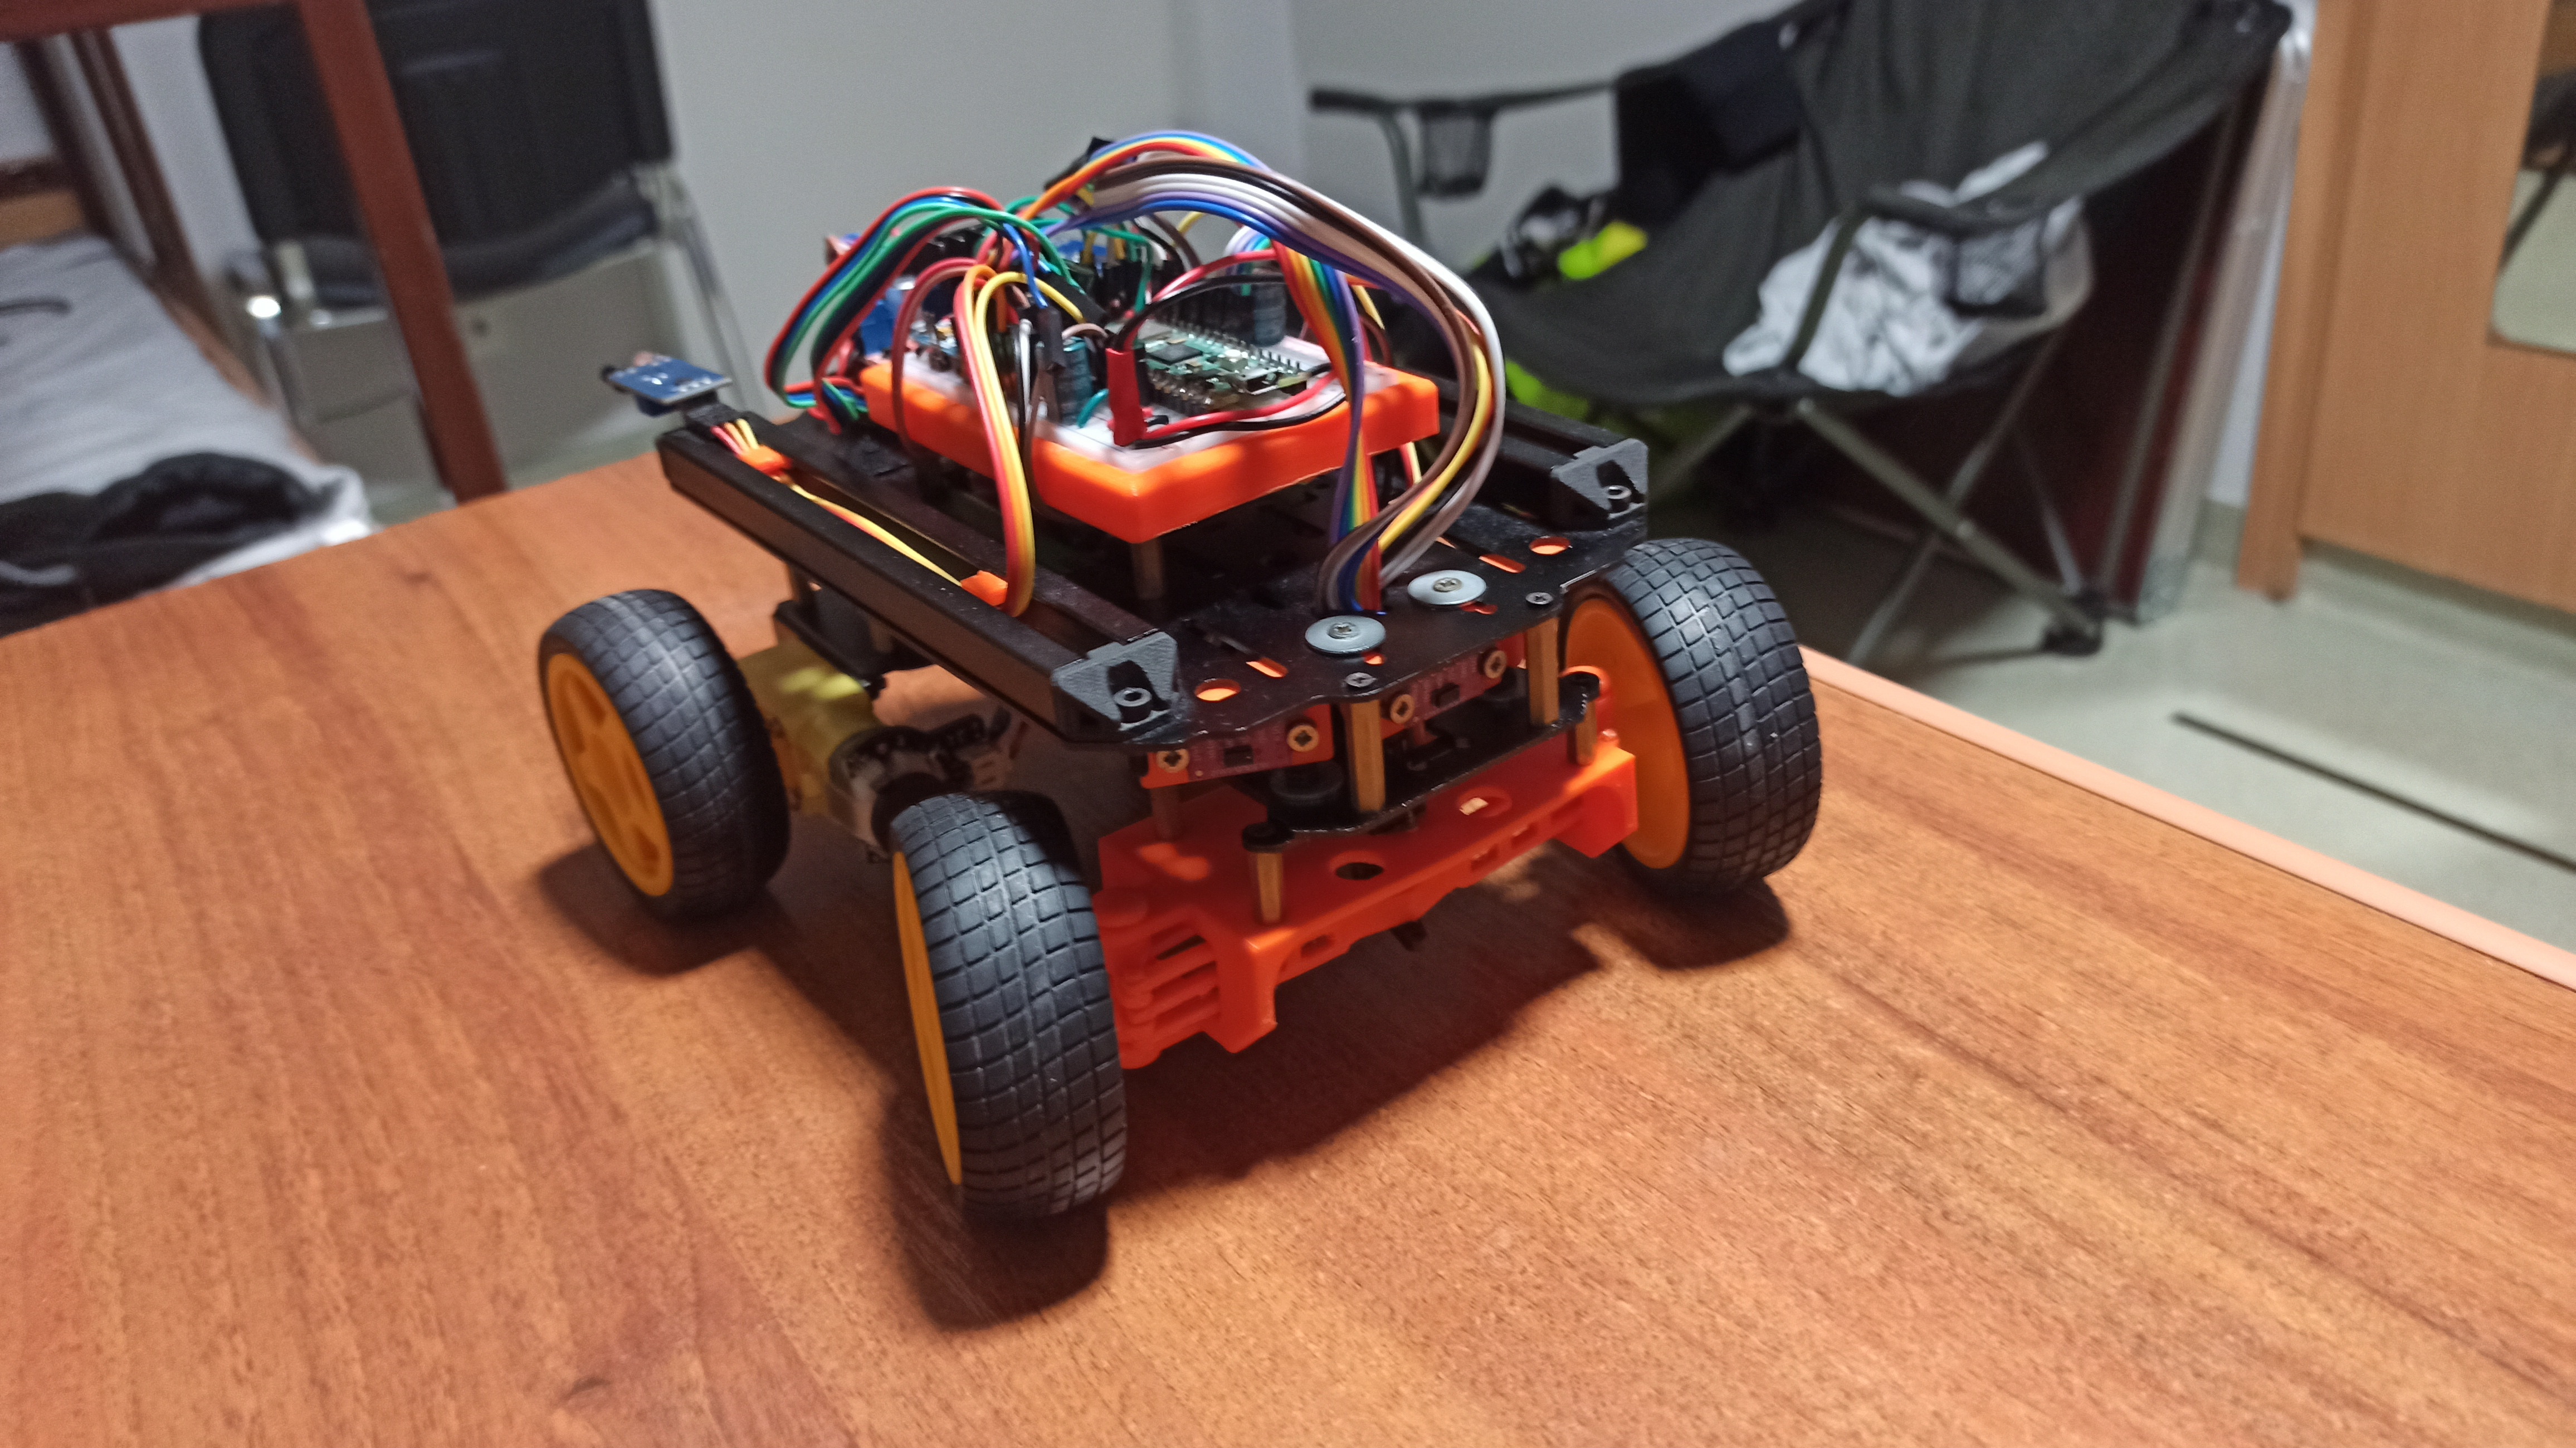
\includegraphics[width = 0.7\textwidth, trim = {800px, 400px, 1200px, 200px}, clip]{Breadboard_car.jpg}
            \caption{Pojazd z zainstalowaną płytą stykową}
            \label{fig:breadboard_car}
        \end{figure}

        Po zamocowaniu płytki do ramy samochód został poddany prostym testom, które polegały na sprawdzeniu działania wszystkich komponentów.
        Następnie zbadano podstawowe funkcje takie jak: jazda prosto czy skręcanie.

        W czasie kontroli poszczególnych elementów pojedynczo, wszystko działało poprawnie.
        Natomiast po dłuższym czasie testy wykazały, że układ akcelerometru potrafi zawiesić się w przypadkowym momencie.
        Jednocześnie zawieszając pracę mikrokontrolera.
        Problematyczna okazała się linia $SDA$ protokołu $I^2C$.
        Jeden z czujników po spadku napięcia, zwierał tę linie do masy, co uniemożliwiało dalszą pracę.

        Pierwszą próbą rozwiązania było zastosowanie się do instrukcji z noty aplikacyjnej od Analog Devices o resetowaniu linii $I^2C$ \cite{application_note_I2C_AD}.
        Podobną sugestię można znaleźć w dokumentacji do tej magistrali \cite{I2C_manual_NXP} wydanej przez NXP.
        Obaj producenci radzą, aby w takiej sytuacji spróbować ręcznie wyczyścić zablokowaną linię danych, wysyłając od 8 do 16 cykli zegara.
        % W ten sposób, zablokowane urządzenie powinno zwolnić linię $SDA$.
        W ten sposób linia $SDA$ powinna zostać zwolniona.
        Niestety przedstawiony mechanizm nie przyniósł oczekiwanych rezultatów.

        Drugim sposobem sugerowanym przez oba dokumenty,
        w sytuacji kiedy nie udało się ustawić magistrali jest zresetowanie niedziałających (w domyśle wszystkich) układów.
        To rozwiązanie mimo swojej skuteczności nie zostało wykorzystane,
        ze względu na bardzo długi czas ponownej inicializacji czujników.
        Autor skupił się na znalezieniu pierwotnej przyczyny, którą okazała się płytka stykowa.
        Podczas jazdy cały pojazd drżał, co powodowało, że niektóre piny nie kontaktowały,
        a w konsekwencji akcelerometr po spadku zasilania, blokował magistralę.
        Zlikwidowanie problemu na tym etapie, okazało się niemożliwe, z powodu działania zastosowanej metody połączeń.
        Jedynym wyjściem było zbudowanie lepszej wersji prototypu.
        % Natomiast kolejny prototyp nie posiadał tego problemu.

        Niespodziewaną zaletą powyższych zmagań było udoskonalenie funkcji odpowiedzialnych za kontrolę protokołu $I^2C$.
        Na początku proces przesyłania danych między czujnikami, blokował pracę całości.
        Czekanie na wynik, sprawdzało się tak długo jak wszystkie moduły odpowiadały poprawnie.
        Jednak luźne połączenia między płytką stykową a pinami elementów ukazały,
        że wstrzymywanie kontrolera do momentu uzyskania odpowiedzi jest niepraktyczne ze względu na blokadę sterowania.
        W ulepszonej wersji kodu dla mikrokontrolera, podczas transmisji danych procesor uwzględnia maksymalny czas na odpowiedź.
        Po przekroczeniu tego limitu, program zgłasza błąd $ERROR\_PICO\_TIMEOUT$, sygnalizujący o niepowodzeniu wymiany informacji.

        Ostatnią testowaną wersją układu jest zlutowana na stałe płytka prototypowa.
        Taka budowa pozwoliła pozbyć się niektórych problemów, przykładowo blokowania się magistrali $I^2C$.
        Jednak i na tym etapie pojawiły się inne mankamenty, które ukrywała płytka stykowa.
        \begin{figure}[!ht]
            \centering
            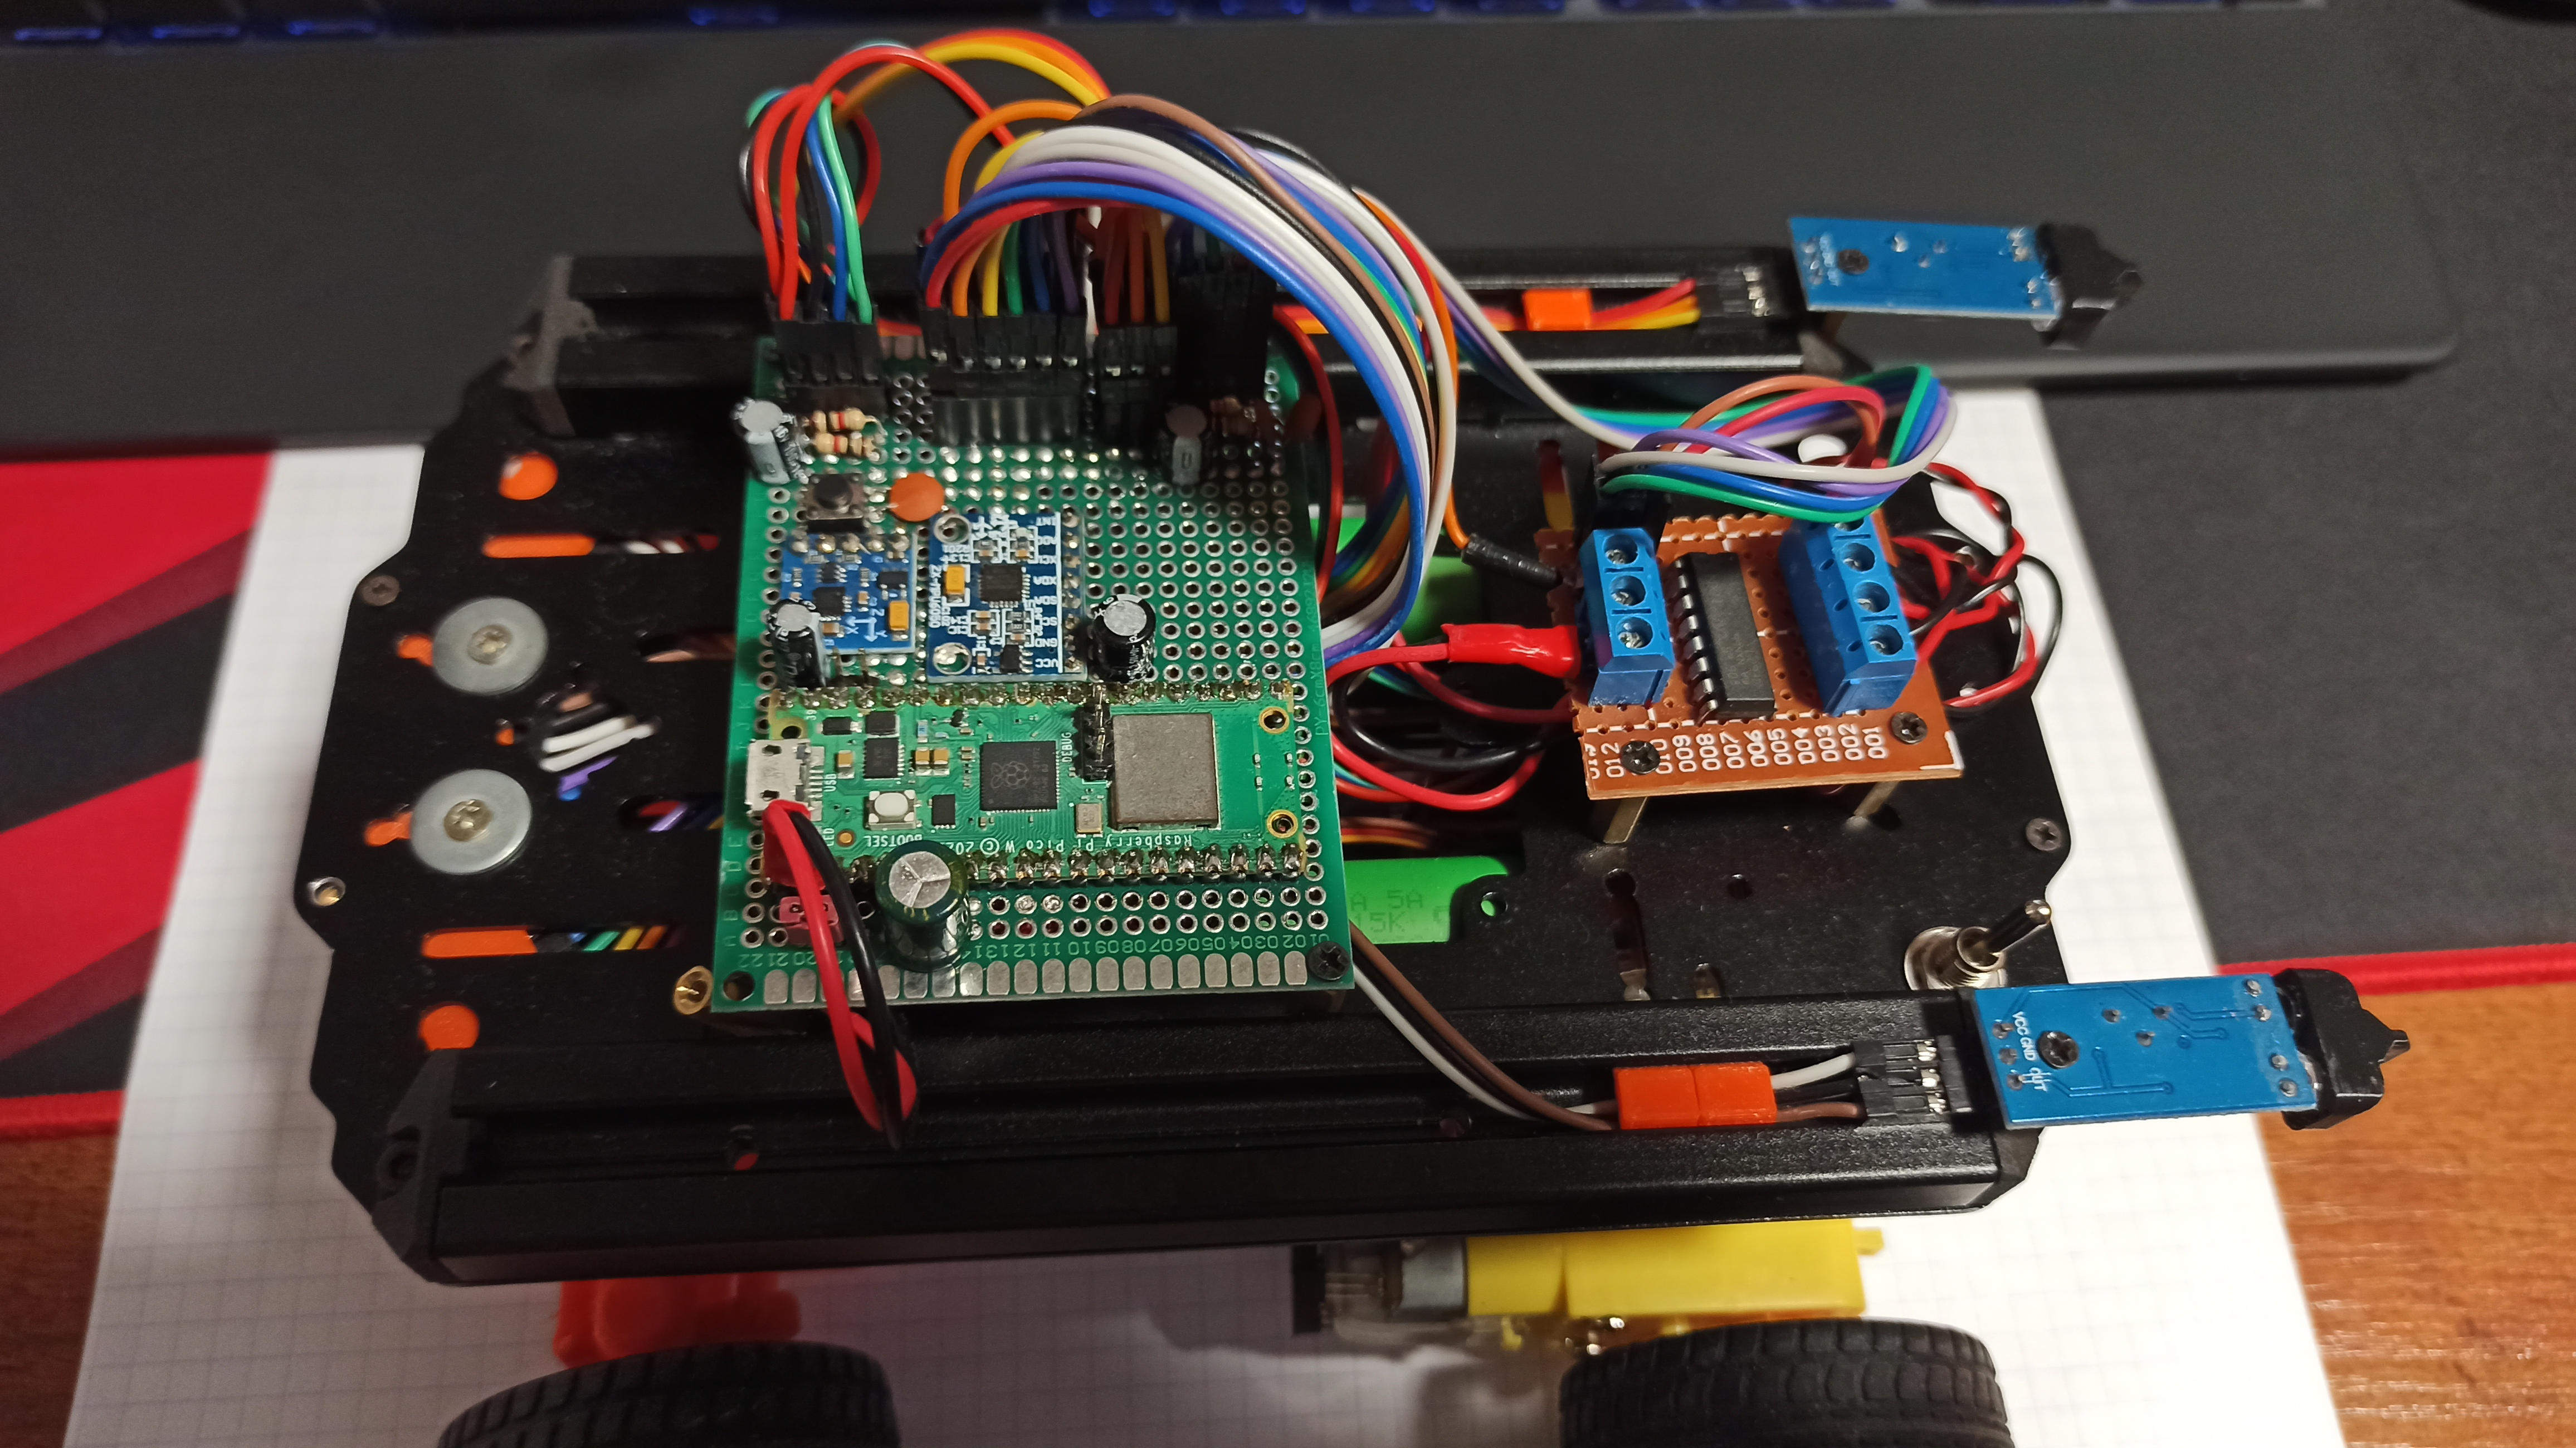
\includegraphics[width = 0.7\textwidth, trim = {500px, 300px, 300px, 200px}, clip]{Protoboard_car.jpg}
            \caption{Model pojazdu z zainstalowaną płytą prototypową}
            \label{fig:protoboard_car}
        \end{figure}

        Największą wadą, która ukazała się podczas testowania tej fazy, było losowe resetowanie się Raspberry Pi Pico.
        Sytuacja ta występowała czasami, zarówno po podłączeniu zewnętrznego zasilacza jak i pracy na akumulatorach.
        Kłopotliwa stała się jednoczesna praca silników i~enkoderów.
        Po odłączeniu wyjść sygnałowych enkoderów, układ przestał się restartować.
        Aby upewnić się, że przyczyną są uszkodzone enkodery, w szeregu z ich wyjściami zostały podłączone rezystory o wartości $1k\Omega$, które chroniły układ przed zwarciem.
        Tak zabezpieczony system powinien pracować poprawnie, jednak restarty nadal występowały.

        Następną próbą było rozseparowanie zasilania.
        W ten sposób silniki zostały podłączone bezpośrednio do zasilacza laboratoryjnego, natomiast Raspberry Pi wraz z pozostałymi modułami do złącza USB.
        Uruchomienie całości w takiej konfiguracji, natychmiast zresetowało procesor.
        Kolejną propozycją była zmiana mostka H na inny, co również nie pomogło.
        Podczas składania prototypu, uszkodzeniu uległ jeden z czujników ToF.
        Po wymianie tego układu, problem nie zniknął.
        Ostatnim co mogło zostać uszkodzone, był sam kontroler, jednak jego wymiana również nie przyniosła oczekiwanego efektu.

        Rozwiązanie okazało się dość prozaiczne.
        Z braku lepszego pomysłu, autor dołożył dużą rozproszoną pojemność (około $500\mu F$) na całej płytce, co okazało się zbawienne dla pracy procesora.


        W tej generacji projektu, uwidoczniły się błędy, wynikające z oscylacji na liniach sygnałowych od czujników obiektów, zamontowanych na tyle pojazdu.
        Drgania te, nie pozwalały na jazdę wstecz, ponieważ układy przy ruszeniu natychmiast zgłaszały przerwanie, a w konsekwencji program zatrzymywał silniki.
        Wyjściem z sytuacji było zastosowanie dolnoprzepustowych filtrów RC, niwelujących spadki zasilania, występujące podczas startu.



    \subsection{Testy automatyczne}
    \label{sec:auto_test}
        Automatyzacja pracy jest niezwykle ważnym zadaniem.
        Istnieje wiele gotowych narzędzi, specjalnie przeznaczonych do tego procesu.
        Autor jednak zdecydował się, na napisanie własnego programu, którego podstawowymi założeniami są: dwukierunkowa komunikacja, zapisywanie odebranych danych do pliku oraz czytanie i wykonywanie podprogramów.
        Dodatkową opcją ma być możliwość wywołania każdej funkcji ręcznie,
        w taki sposób, aby całość była przejrzysta dla użytkownika - proces analizy kodu i pracy manualnej, nie powinien wymuszać każdorazowego uruchomienia aplikacji.

        Aby wykonać to zadanie, w języku Python został napisany skrypt, który pozwala na dwustronną transmisję za pomocą protokołu $UDP$.
        Dzięki temu użytkownik może wysyłać komendy do mikrokontrolera, a równocześnie program nasłuchuje odpowiedzi i wyświetla wyniki.
        Co więcej instrukcja $file\ \{path\}$ pozwala na interpretację podprogramów, napisanych wyłącznie dla tego układu.
        Przykład takiego kodu przedstawiono na listingu \ref{list:self_test.s}.
        % Poniżej w listingu \ref{list:self_test.s} przedstawiono przykład kodu do testowania pojazdu.

        \lstinputlisting[style=asm, caption={Test pojazdu}, label = list:self_test.s]{Listing/self_test.s}

        \subsubsection{Interpreter własnego języka}
            Przedstawiony kod (listing \ref{list:self_test.s}) jest interpretowany, przez wyżej wymieniony skrypt (rozdz. \ref{sec:auto_test}).
            Działanie interpretera polega na: sformatowaniu instrukcji, wyznaczaniu adresów skoków oraz stworzeniu słownika ze zmiennymi.
            Następnie program przechodzi do wykonywania poleceń, zapisanych w pliku.
            Powyższy język posiada tylko kilka słów kluczowych, przedstawionych w~tabeli~\ref{table:keywords}.

            \begin{table}[!ht]
                \centering
                \caption{Lista słów kluczowych do mini języka}
                \begin{tabularx}{0.8\textwidth}{|c|c|C|}\hline
                    Nr. & Instrukcja & Opis \\\hline
       \centerY{2}{ 1.} & \centerY{2}{$etykieta$\textbf{:}} & Etykieta funkcji, koniecznie zakończona znakiem ,,:''\\\hline
                     2. & jump $etykieta$ & Skok do $etykiety$ \\\hline
                     3. & end & Koniec programu lub funkcji \\\hline
                     4. & print $zmienna/napis$ & Wypisanie wartości zmiennej lub napisu\\\hline
       \centerY{2}{ 5.} & \centerY{2}{if $warunek$} & Instrukcja warunkowa, w przypadku niespełnienia pomija następną instrukcję\\\hline
       \centerY{3}{ 9.} & \centerY{3}{$\$zmienna$} & Odwołanie do zmiennej. Podczas formatowania polecenia, $\$zmienna$ zostaje podmieniona na wartość\\\hline
       \centerY{3}{10.} & \centerY{3}{$zmienna$ = \textit{wartość}} & Przypisanie wartości do zmiennej. Pozwala na wykonywanie operacji matematycznych\\\hline
       \centerY{1}{11.} & \centerY{1}{$zmienna$ == $zmienna$} & Porównanie dwóch wartości\\\hline
       \centerY{2}{12.} & \centerY{2}{sleep $zmienna$} & Zatrzymaj wykonywanie kodu na czas ze~$zmiennej$\\\hline
                \end{tabularx}
                \label{table:keywords}
            \end{table}

            Wszystkie pozostałe instrukcje, które nie są zdefiniowane w tabeli \ref{table:keywords}, ulegają formatowaniu i wysłaniu do mikrokontrolera.
            W celu ich wyróżnienia, w konsoli bezpośrednio przed nimi zostaje wyświetlony łańcuch ,,$>>>$''.
            % W celu rozróżnienia komend wysyłanych do pojazdu a tych odebranych w trakcie interpretacji kodu, polecenia  poprzedzone są łańcuchem znaków ,,$>>>$''.
            Natomiast odebrane dane i wyniki polecenia $print$ są identyczne i niepoprzedzone żadnym znacznikiem.
            % Natomiast wynik polecenia $print$ jest identyczny z tym, co zwraca Raspberry Pi Pico.

            W przypadku kiedy dyrektywa zostaje odnaleziona, ale zawiera błąd składniowy, program wypisuje informacje o napotkanym problemie i przerywa działanie.
            Przykład takiej sytuacji przedstawiono na zdjęciu poniżej (rys. \ref{fig:interpreter}).

            \begin{figure}[!ht]
                \centering
                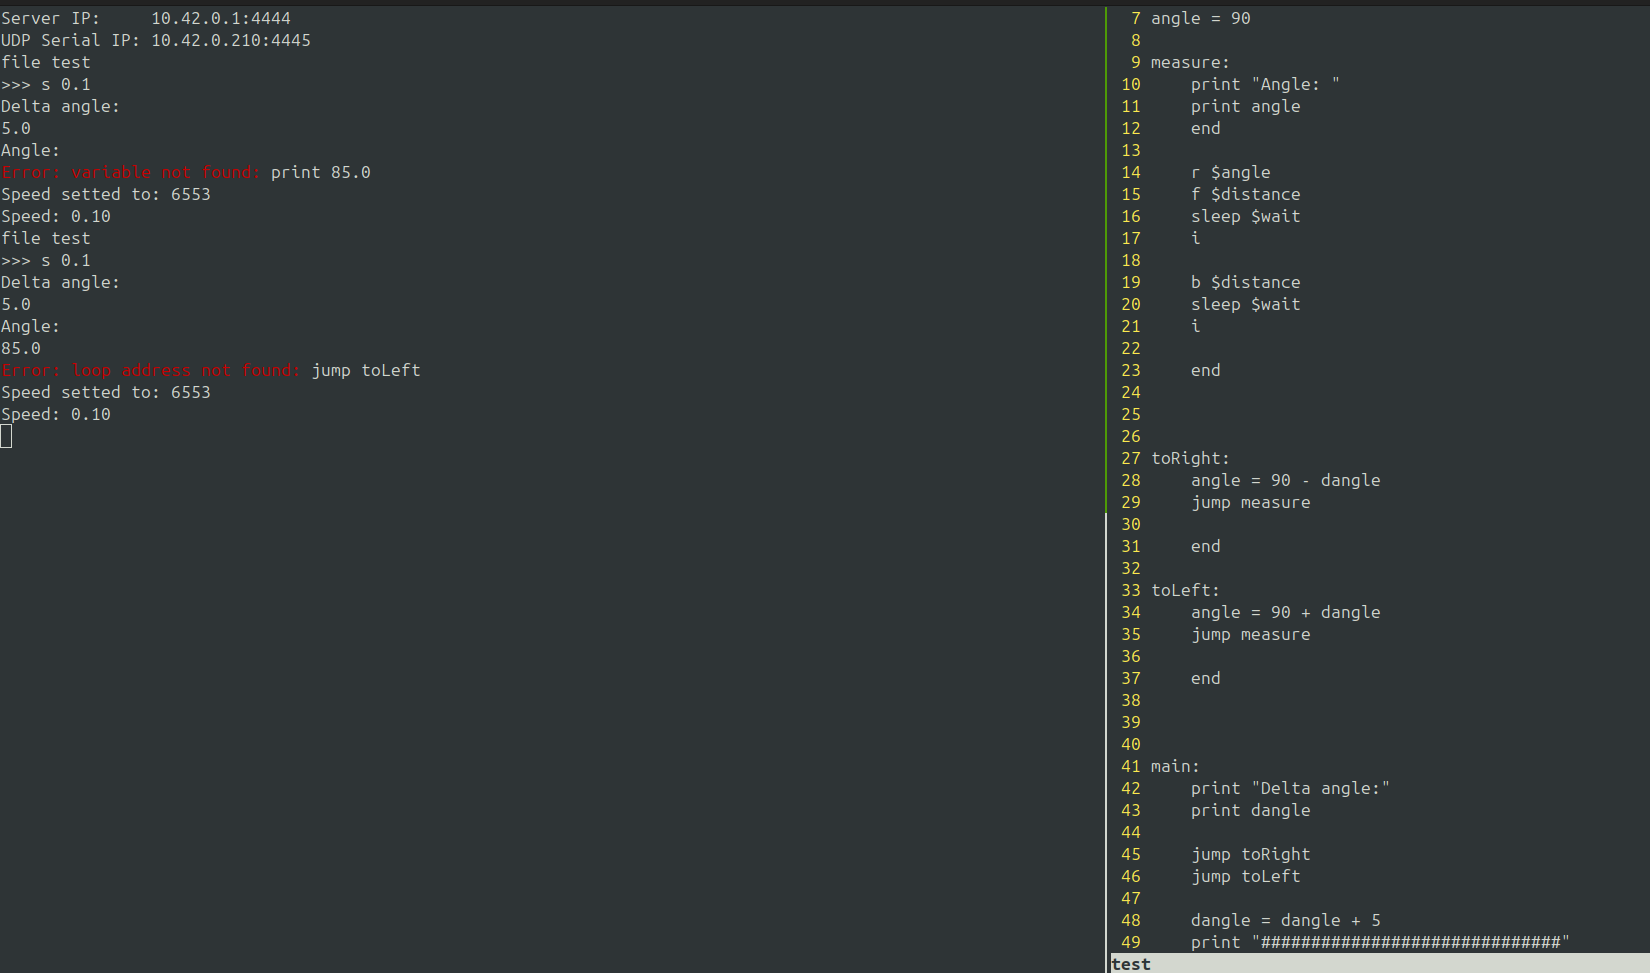
\includegraphics[width = \textwidth]{Terminal_program_testowy.png}
                \caption{Program zawierający celowe błędy}
                \label{fig:interpreter}
            \end{figure}

            Praca interpretera jest równoległa z odczytywaniem danych, dlatego zdarza się, że pomimo niepowodzenia program wyświetla wynik ostatniej poprawnej operacji.
            Taka sytuacja wystąpiła na rysunku \ref{fig:interpreter}. Skrypt zdążył wysłać kilka poleceń do Raspberry, następnie natrafił na błąd składniowy, co zatrzymało proces.
            W tym czasie ostatnia wykonana instrukcja zwróciła wartość, a program wyświetlił jej wynik.

\newpage
\